\section{Plazierung am Markt} % (fold)
\label{sec:plazierung_am_markt}

\subsection{Marktanalyse: Welche Communities gibt es schon?} % (fold)
\label{sub:marktanalyse_welche_communities_gibt_es_schon}
Für Studierende an der AKAD–University gibt es eine Reihe von Angeboten im Internet, die einzelne Elemente der in Kapitel~\myref{sub:zusammenspiel_der_werkzeuge} beschriebenen \ac{cscl}–Umgebung abdecken. Diese werden zum Teil bereits heute von der AKAD–University bereitgestellt, wie etwa die Materialien zum Selbststudium, Lernvideos und eine Diskussionsfunktion auf Ebene der Studienmodule. Letztere bietet allerdings nicht die für ein Forum notwendige Übersichtlichkeit und eignet sich somit nicht als Ersatz für ein Forum.\footnote{vgl. \cite{defstud}, Abschnitt „Moduldiskussion / Studienbetreuung“}

Zum Austausch zwischen den Studierenden stehen mit \buzz{Fernstudenten.de}\footnote{Öffentliche Beiträge. Zum Einstellen von Inhalten ist ein Benutzerkonto notwendig. Die Hochschulzugehörigkeit wird jedoch nicht geprüft. Siehe \url{Fernstudenten.de}} und einem Netzwerk an \buzz{Facebook–Gruppen}\footnote{Beiträge nur für Gruppenmitglieder einsehbar. Die Hochschulzugehörigkeit wird oberflächlich geprüft. Dozenten und Mitarbeiter der Hochschule werden nicht zugelassen. Siehe \url{facebook.com/groups/AKADStudentengruppe/}} unabhängige Angebote zur Verfügung.

Bei Fernstudenten.de werden neben Fragen zum Studienablauf auch Gedächtnisprotokolle von Klausurstellungen und von Studierenden erstellte Zusammenfassungen des Lernstoffs oder andere Lernhilfen ausgetauscht. Der Charakter der Kommunikation ist hierbei asynchron mit langen Beiträgen und Diskussionen die sich über Tage und Wochen hinziehen. In den Facebookgruppen werden neben aktuellen Fragen zum Studienablauf auch Hinweise auf Zeitschriftenartikel, Lernmaterialien und anderes veröffentlicht. Der Charakter der Kommunikation ist hierbei eher synchron mit meist kurzen Beiträgen und Diskussionen die meist nach einigen Stunden oder innerhalb weniger Tage abgeschlossen sind.
Die Studierendenvertretung nutzt sowohl Fernstudenten.de als auch die Facebookgruppen als Kontaktmedium zu den Studierenden.

Audio– und Videovorlesungen sowie weitere Lernmaterialien stehen online von vielen Anbietern\footnote{z.B. die im \buzz{\ac{OEC}} oder auch bei \buzz{iTunes U} zusammengeschlossenen Universitäten} sowohl auf eigenen Plattformen\footnote{z.B. Hasso Plattner Institut (\url{open.hpi.de}) oder Harvard (\url{cs50.harvard.edu/})} sowie auf Videoportalen\footnote{z.B. YouTube (\url{YouTube.com}) oder Vimeo (\url{Vimeo.de})} zur Verfügung.
% subsection marktanalyse_welche_communities_gibt_es_schon (end)

\subsection{Alleinstellungsmerkmale} % (fold)
\label{sub:alleinstellungsmerkmale_plazierung}
Ein Alleinstellungsmerkmal der AKAD–University ist das Angebot von anerkannten akademischen Abschlüssen bei individueller und absolut freier Festlegung der Lernzeiten durch den Studierenden. Auch die Prüfungsleistungen sind im Rahmen der angebotenen Termine frei wählbar. Eine Beschränkung der Studienzeit besteht laut \ac{SPO} nicht. Konkurrenzangebote sind entweder an Semester gebunden\footnote{z.B. \ac{LINAVO} oder ERP4students} oder die Abschlüsse sind nicht staatlich oder zumindest in der Wirtschaft allgemein anerkannt.

Durch die Ausrichtung des Lernangebots auf eine anerkannte \ac{SPO} sowie durch die Betreuung des Lernvorgangs durch hochschuleigene Dozenten wird eine entsprechende Lernplattform trotz alternativer Angebote von den Studierenden genutzt werden. Die \ac{CSCL}–Plattform wird als integraler Bestandteil des Studienangebots und der Leistung der AKAD–University wahrgenommen werden und zentrale Aufgaben im akademischen und organisatorischen Bereich unterstützen.
% subsection alleinstellungsmerkmale_plazierung (end)

\subsection{Struktur} % (fold)
\label{sub:struktur}
Aufgrund der Modulorientierung der Studiengänge bietet sich grundsätzlich eine ebendiesen Studienmodulen orientierte Gliederung aller \ac{CSCL}–Werkzeuge in entsprechende Bereiche\footnote{je nach Werkzeug können dies Foren, Speicherordner im Videoportal oder Themenbereiche im Wiki bzw. der Wissensbasis sein.} an. Die Zugriffsmöglichkeiten sollten hierbei jedoch flexibel über Schlagworte möglich sein. Dies ermöglicht den individuellen Zugriff der Teilnehmer über die jeweils passenden Pfade. 

So könnte z.B. das Modul \buzz{DBA02} einerseits direkt (\code{/DBA02}), über den Studiengang (\code{/Sc/Bachelor/WInf/3.Semester/Datenbanksysteme/DBA02}), über die im Modul besprochenen Inhalte (\code{/OOP/PHP/SQL/DBA02}) oder auch über den Studienfortschritt des Lernenden (\code{/MeineModule/Fertig/Note<2,3}) erreicht werden. Das Nutzerinterface sollte also als Filter auf Basis von Taxonomien und nicht als Darstellung fester Hierarchien implementiert werden.\footnote{Somit sind dann auch kürzere oder gemischte Zugriffspfade wie etwa \code{/SQL/3.Semester/DBA02} möglich.} Wie im letzten Beispiel ersichtlich, sollten hier sowohl allgemein gültige als auch für jeden Teilnehmer individuelle Taxonomien sowie Schlüssel–Wert–Paare unterstützt werden.

Neben den modulbezogenen Bereichen werden noch weitere, modulübergreifende Bereiche benötigt. Hier können dann Lerninhalte über Modulgrenzen hinweg miteinander verknüpft werden, oder Themen besprochen werden, die nicht in direktem Zusammenhang mit den Lerninhalten stehen, aber für das Studium relevant sind. Beispiele hierfür sind individuelle Lerngruppen\footnote{vgl. \cite{cscl:wessner}, Seite 200ff}, die organisatorische Studienbetreuung, die Aktivitäten der Studierendenvertretung, Kommunikation zwischen Dozenten und Ähnliches. Die Ausweitung auf extracurriculare Aktivitäten ist denkbar, aber aufgrund der begrenzten Zahl an Studierenden sowie anderer, themenspezifischer\footnote{z.B. \url{Forum.Fluegelvieh.de}} oder allgemeiner\footnote{z.B. \url{Facebook.com}} Plattformen nicht notwendig.
% subsection struktur (end)

\subsection{Nutzung \& Reichweite} % (fold)
\label{sub:reichweite}
Die Nutzerbasis sollte auf die Mitglieder und Angehörige der AKAD University\footnote{Dies umfasst alle an der AKAD–University beschäftigten akademischen und nicht–akademischen Mitarbeiter sowie die immatrikulierten Studierenden, vgl. \cite{akad:go}, §3 Absatz 1 \& 3} und deren Alumni beschränkt sein, um ein Mindestmaß an Verbundenheit zur Hochschule zu gewährleisten. 

Für Lerngruppen sollte die Möglichkeit bestehen, ihren Bereich nur für Mitglieder der Lerngruppe zugänglich zu machen, um die für solche Gruppen notwendige Vertrautheit zu erzeugen und dadurch die gewünschten Eigenschaften von kooperativen Lerngruppen wie positive Abhängigkeit, persönliche Verantwortung, fördernde Interaktion soziale Kompetenz und Reflexion der Gruppenarbeit zu fördern.\footnote{vgl. \cite{cscl:wessner}, Seite 201f}

Einige wenige Bereiche wie die Studienberatung können auch für die Allgemeinheit geöffnet werden. Da diese Bereiche dann auch Suchmaschinen zugänglich sind, besteht hier auch Potential für die Kommunikation zu potentiellen Studierenden und somit zur Neukundengewinnung.
% subsection reichweite (end)

\subsection{Rechtesystem} % (fold)
\label{sub:rechtesystem}
Die Authorisierung der Nutzer geschieht über das vorhandene Login des \ac{OCS}, gegebenenfalls über entsprechende Schnittstellen. Aus dieser Benutzerverwaltung kommen auch Informationen über die Rollen und Rechte des jeweiligen Nutzers. 

So sollen Studierende im Forum die ihrem Studiengang zugeordneten Module sowie die allgemeinen Bereiche einsehen und dort Beiträge erstellen, kommentieren und beantworten können. Sie sollen Lerngruppen beitreten können oder diese erstellen dadurch Verwalter dieser Gruppe werden. Gruppenverwalter können das Thema der Gruppe bestimmen und andere Teilnehmer zur Teilnahme einladen und wieder entfernen. Nach dem Erreichen des Gruppenziels kann diese archiviert werden, so dass keine weitere Bearbeitung möglich ist. Der Gruppenverwalter ist für die Einhaltung der Umgangsformen und der rechtlichen Bestimmungen innerhalb seiner Gruppe verantwortlich und kann daher dort auch Beiträge anderer Teilnehmer ausblenden bzw. löschen. In den Modulbereichen übernehmen die Dozenten oder Moderatoren diese Aufgabe.

Diese Grundfunktionen und Rechte sind bei den unterschiedlichen Werkzeugen des \ac{CSCL} unterschiedlich ausgestaltet. Beim Wiki werden im Vergleich zum Forum umfangreichere Rechte eingeräumt. So kann dort jeder Nutzer die Beiträge der anderen Ändern und sogar löschen, da dies zur Grundfunktionalität von Wikis gehört und es durchaus üblich ist, dass vorhandene Wikiseiten von mehreren Autoren stark bearbeitet und z.T. ganze Bereiche des Wikis mit mehreren Seiten umstrukturiert werden, um die Qualität zu erhöhen. 

Bei der Wissensbasis und den Lernunterlagen gilt das Gegenteil: Hier sind sämtliche Eintragungen durch einen entsprechenden Qualitätssicherungsprozess zu überwachen und nur nach offizieller Prüfung frei zu schalten. Selbst Änderungen von Dozenten sollten hier erst nach einem Review in die offizielle Version eingehen.\footnote{siehe auch Abschnitt~\myref{sub:reviews}}
% subsection rechtesystem (end)
% section plazierung_am_markt (end)

\section{Technische und wirtschaftliche Aspekte} % (fold)
\label{sec:technische_und_wirtschaftliche_aspekte}

\subsection{Benötige Hard- und Software} % (fold)
\label{sub:benotige_hard_und_software}
Die konkrete benötigte Software hängt von Entscheidungen ab, die in dieser Arbeit nicht weiter betrachtet werden, wie z.B. ob eine hochintegrierte Lösung individuell erstellt wird, oder ob vorhandene Systeme integriert werden sollen. Aufgrund der Textlastigkeit der Werkzeuge sind mit üblicher Hardware auch große Nutzergruppen handhabbar, so lange diese Werkzeuge nur schwach integriert sind.\footnote{vgl. z.b \cite{phpbblarge} für Foren oder \cite{dwlarge} für Wikis}

Für höhere Integrationsanforderungen sollten genauere Tests und Anforderungsanalysen durchgeführt werden.
% subsection benotige_hard_und_software (end)

\subsection{Benötigte Schnittstellen} % (fold)
\label{sub:benotigte_schnittstellen}
Die für die Integration wichtigste Schnittstelle ist die zur Benutzerverwaltung des \ac{OCP}. Die Studierenden sollen sich mit einem Benutzernamen und Passwort beim System anmelden. Dieses Login soll dann auch für alle Teilsysteme und CSCL–Werkzeuge gültig sein.

Um die Anfragen der Studierenden mit dem \ac{TTS} überwachen zu können, ist eine Schnittstelle vom Forum zum \ac{TTS} notwendig, die bei neuen Fragen entsprechende Vorgänge erzeugt und bei Antworten auf Fragen diese je nach Rolle und Status des Antwortenden bzw. durch entsprechende Schlüsselworte in der Diskussion den Status der erzeugten Vorgänge ändert.

Ebenso ist eine Schnittstelle zwischen dem Wiki und der Wissensbasis wünschenswert, über die ein Review-- und Integrationsprozess unterstützt wird.\footnote{vgl. \cite{governor}, Abschnitt „The Participation-Collaboration Pattern“}

Rechtssicherheit und Qualität lassen sich durch eine Schnittstelle zwischen Wiki bzw. Wissensbasis und einem System zur automatischen Prüfung auf Plagiate erhöhen. Über die gleiche Schnittstelle könnten auch weitere Textanalysen durchgeführt werden, welche die Inhalte automatisch verschlagworten könnte.
% subsection benotigte_schnittstellen (end)

\subsection{Integration mit vorhandenen Systemen} % (fold)
\label{sub:integration_mit_vorhandenen_systemen}
Die einzelnen Teilsysteme haben sich optisch in das Vorhandene \ac{OCP} einzugliedern. Ein schnelles, beutzerfreundliches Wechseln zwischen den einzelnen Werkzeugen soll möglich sein. Benachrichtigungen über Reaktionen auf eigene Beiträge sollten über ein einheitliches System, werkzeugübergreifend zugestellt werden.
% subsection integration_mit_vorhandenen_systemen (end)

\subsection{Benötigtes Budget} % (fold)
\label{sub:benotigtes_budget}
Es müssen Mittel für die Entwicklung und für den Betrieb bereitgestellt werden. Bei der Realisierung als Individualsoftware sind die Entwicklungskosten im Vergleich zu Standartkomponenten höher. Aber auch die Integration von fertigen Teilsystemen muss im Budget berücksichtigt sein. Diese Kosten treten nicht regelmäßig auf, sondern lediglich vor der Einführung, während des Customizing sowie bei Updates auf.

Die Kosten für Server und Lizenzen stellen einen Teil der laufenden Kosten dar, dessen größter Teil allerdings in den Personalkosten für die technische, organisatorische sowie akademische Betreuung des Angebots ausmacht.

% subsection benotigtes_budget (end)

\subsection{Demand Management im CSCL} % (fold)
\label{sub:demand_management}
Um die gegebenen personellen Resourcen möglichst effizient einsetzen zu können, kann ein Demand Management System eingesetzt werden, welches den Großteil der täglichen Anfragen der Lernenden durch Tutoren\footnote{z.B. Studierende aus höheren Semestern, die das entsprechende Modul bereits bearbeitet haben} beantworten lässt, welche komplizierte Fragen im Bedarfsfall die Dozenten bzw. Professoren oder bei Verwaltungsfragen  die zuständigen Mitarbeiter auf die Probleme aufmerksam macht.\footnote{Übertragung des Prinzips „Demand Management“ aus dem Gesundheitswesen, vgl. \cite{gabler:demandmanagement} in den Kontext des Fernstudiums \cite{ojstersek}, Seite 127}
% subsection demand_management (end)

% section technische_und_wirtschaftliche_aspekte (end)

\section{Redaktionelles Konzept} % (fold)
\label{sec:redaktionelles_konzept}
\subsection{Forum als Werkzeug für Dozenten} % (fold)
\label{sub:forum_als_werkzeug_fur_dozenten}
Das Forum bietet den Dozenten die Möglichkeit, aktiv mit den Studierenden in Kontakt zu treten. So können in regelmäßigen Abständen (z.B. wöchentlich) ergänzende Informationen zu den Lernmaterialien eingestellt und zur Diskussion aufgerufen werden. Durch die Forendiskussion werden eventuelle Unklarheiten in den Lernvideos oder Lernmaterialien deutlich und diese können entsprechend präzisiert werden. Fragen der Studierenden sollten innerhalb eines möglichst kurzen Zeitraums beantwortet werden. Sollte eine Studierendenfrage nach dem Schema aus Abbildung~\ref{fig:wuerfel} als „nicht dringend“ aber mit „hohem pädagogoischem Potential“ eingestuft werden, so sollte dies den Lernenden mitgeteilt und eine entsprechende Diskussion angestoßen werden.
% subsection forum_als_werkzeug_fur_dozenten (end)

\subsection{Forum als Werkzeug für Studierende} % (fold)
\label{sub:forum_als_werkzeug_fur_studierende}
Studierende können das Forum als Fragemöglichkeit nutzen, mit der sie die Dozenten kontaktieren können. Die öffentlichen Fragen und Antworten helfen auch Studierenden, die den jeweiligen Sachverhalt nicht genug beachtet haben um die Frage selbst zu stellen, aber auch denjenigen, die das Problem gelöst haben und eine Antwort beisteuern können. Hierdurch wird nämlich das gelernte mit eigenen Worten formuliert und somit gefestigt.

Außerdem können Themen des Studienablaufs und Fernstudienalltags diskutiert werden, wie dies bereits in den vorhandenen Communities auch der Fall ist.
% subsection forum_als_werkzeug_fur_studierende (end)

\subsection{Aufgabe des Monats} % (fold)
\label{sub:aufgabe_des_monats}
Die Interaktion zwischen den Studierenden kann auch dadurch gefördert werden, dass in regelmäßigen Abständen die Lernenden sich gegenseitig Aufgaben stellen. Durch den Perspektivwechsel beschäftigen sich die Aufgabensteller sehr intensiv mit den Thema und auch die Befragten profitieren von neuen Aufgabenstellungen, die von den Aufgaben in den Lernmaterialien abweichen.

Die Aufgaben können modulspezifisch oder –übergreifend gestellt werden. Dafür sollte ein spezieller Bereich des Forums genutzt werden. Impulse für mögliche Themenfelder sollten von den Dozenten ausgehen. Es kann durchaus dazu angeregt werden, eine ausgefallene Aufgabenstellung zu wählen.\footnote{vgl. \cite{dmark}}
% subsection aufgabe_des_monats (end)

\subsection{Forum als Kommunikationsmedium der Betreuung} % (fold)
\label{sub:forum_als_kommunikationsmedium_der_betreuung}
Die Abwicklung von Anfragen an die Studienbetreuung in einem für alle Studierenden einsehbaren Forum ermöglicht es, sich wiederholende Fragen auf ein Minimum zu reduzieren. Die Suchfunktion des Forums kann im Erfolgsfall die Anwortzeit von Stunden oder Tagen auf wenige Sekunden verringern. Um hier die notwendige Qualität der Antworten sicherstellen zu können ist es notwendig, dass die Antworten auf Anfragen tatsächlich von Mitarbeitern der Studienbetreuung gegeben, oder zumindest bestätigt werden.

Durch die Arbeit im Forum werden wiederkehrende Problemstellungen offensichtlich und können über das Wiki zu \ac{FAQ}s die in die Wissensbasis eingehen weiterverarbeitet werden.
% subsection forum_als_kommunikationsmedium_der_betreuung (end)

\subsection{Nutzung in der Studierendenvertretung} % (fold)
\label{sub:nutzung_in_der_studierendenvertretung}
Die Kombination von Forum, Wiki, Wissensbasis und einer von der Hochschule als authentisch bestätigten Menge an Nutzern ermöglicht gezielte und offene Kommunikation zwischen den Studierenden untereinander sowie mit ihren gewählten Vertretern. Probleme können offener angesprochen werden, als dies auf öffentlich zugänglichen und von Suchmaschinen erfassten Plattformen möglich bzw. wünschenswert wäre. Durch die Integration in die Lernplattform ist auch sichergestellt, dass alle Studierenden an der Diskussion teilnehmen können, ohne sich bei hochschulfremden Diensten anmelden zu müssen.
% subsection nutzung_in_der_studierendenvertretung (end)

\subsection{Wiki--Seiten und Wissensbasis} % (fold)
\label{sub:wiki_seiten_zur_zusammenarbeit}
Wenn eine Forendiskussion sich über mehrere Beiträge hinweg entwickelt, kann es hilfreich sein, die von unterschiedlichen Personen beigesteuerten Teillösungen in einer oder mehreren Wikiseiten zu strukturieren und konsolidieren. Hierbei kann die Zusammenarbeit an einem gemeinsamen Text eingeübt werden. Die hier entstehenden Texte können bei entsprechender Qualität das Fundament für neue Artikel in der Wissensbasis dienen. Ebenso können Artikel der Wissensbasis ins Wiki kopiert werden, um dort gemeinschaftlich daran arbeiten zu können.
% subsection wiki_seiten_zur_zusammenarbeit (end)

% section redaktionelles_konzept (end)

\section{Qualitätssicherung} % (fold)
\label{sec:qualitatssicherung}

\subsection{Incentive-System} % (fold)
\label{sub:incentive_system}
Ein einfaches Mittel zur Qualitätsicherung auf sozialer Basis ist die Implementierung eines Anreizsystems, welches die intrinsische Motivation zum Wissenstransfer stärkt. Dies können die im Kapitel~\myref{sec:best_practice} beschriebenen Verfahrens der Punktevergabe durch Peers oder des Erarbeitens von Expertenstatus sein.

Ein extrinsisches Anreizsystem ist durch die Möglichkeit über die Mitarbeit im \ac{CSCL}–Portal echte \ac{ECTS} Credits erwerben zu können gegeben. Dies könnte dadurch umgesetzt werden, dass ein Testat, welches die erfolgreiche Teilnahme am Modul „Schlüsselqualifikationen: Lerntechniken“ nur dann ausgestellt wird, wenn eine zuvor bestimmte Anzahl von Beiträgen im \ac{CSCL}–System durch den jeweiligen Lernenden erstellt wurden. Eventuell müsste für diese Form des Anreizes die entsprechende Modulbeschreibung oder die \ac{SPO} geändert werden.\footnote{vgl. \cite{beuth:anreiz}, Abschnitt „Anreizsysteme im Wissensmanagement“}
% subsection incentive_system (end)

\subsection{Meldesystem} % (fold)
\label{sub:meldesystem}
Über ein Meldesystem sollen alle Teilnehmer einzelne Beiträge, die nicht den Ansprüchen der Gemeinschaft entsprechen melden können. Die kann im Fall von schlecht recherchierten Fragen oder Antworten durch die Vergabe von „Downvotes“ geschehen, oder durch eine spezielle Funktion zum Melden von Beiträgen, die illegale Inhalte aufweisen. Nachdem die Beiträge von Teilnehmern gemeldet wurden, werden diese zunächst nicht mehr angezeigt, bis ein Administrator sie begutachtet und über den weiteren Verbleib des Beitrags entschieden hat. Mögliche Maßnahmen sind leichte Umformulierungen, die Streichung von einzelnen Passagen bis hin zur vollständigen Löschung des Beitrags oder im Extremfall die Weitergabe an Ermittlungsbehörden.

Wichtig ist jedoch, dass bereits die Meldung eines Teilnehmers zu einer schnellen offiziellen Reaktion führt, um Auswirkungen auf die Gemeinschaft möglichst gering zu halten.
% subsection meldesystem (end)

\subsection{Automatische Prüfungen} % (fold)
\label{sub:prufung_auf_plagiate}
Über die in Abschnitt~\myref{sub:benotigte_schnittstellen} beschriebenen Schnittstellen lassen sich automatische Prüfsysteme in den Veröffentlichungsprozess einbinden. So kann schon während der Eingabe die Rechtschreibung geprüft werden. Ebenso ist die automatische Prüfung auf Plagiate möglich. Wie beim manuellen Meldesystem so ist auch bei der automatischen Prüfung eine schnelle Prüfung durch qualifizierte Mitarbeiter notwendig.
% subsection prufung_auf_plagiate (end)

\subsection{Reviews} % (fold)
Zusätzlich zu den automatischen oder auf dem sozialen Netzwerk basierenden Möglichkeiten der Qualitässicherung ist zumindest für Änderungen oder Ergänzungen in der Wissensbasis oder in den Lernmaterialien zusätzlich eine Begutachtung mit dem ausdrücklichen Ziel der Qualitätssicherung notwendig. Die genannten Felder bilden die Grundlage für die Lehre der Hochschuld und Änderungen daran sollten entsprechend sorgfältig gehandhabt werden.

\label{sub:reviews}
\begin{figure}[H]
\begin{center}
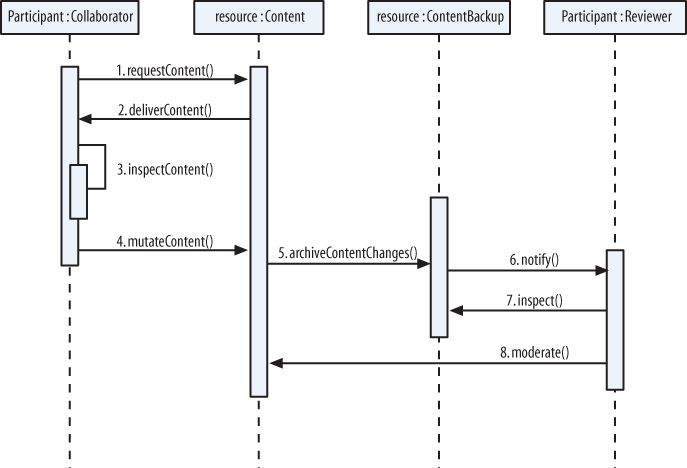
\includegraphics[width=\textwidth]{partcollpat.png}
\caption[Das Participation–Collaboration Pattern]{Das Participation–Collaboration Pattern\footnotemark}
\label{fig:partcolpat}
\end{center}
\end{figure}
\footnotetext{\cite{governor}, Abschnitt „The Participation-Collaboration Pattern“}
% subsection reviews (end)

Durch die Implementierung des \buzz{Participation-Collaboration Patterns} wird eine unkomplizierte Veränderung der Inhalte ermöglicht. Die neue, veränderte Version wird allerdings erst dann der Allgemeinheit angezeigt, wenn ein Reviewer diese auch bestätigt hat. Reviewer sollten die notwendige Sachkenntnis haben, um die Qualität der Beiträge überprüfen zu können.  Da davon auszugehen ist, dass die Rolle der Reviewer unter anderem von Dozenten oder anderen Lerngruppenteilnehmern wahrgenommen wird, sollte sicher gestellt werden, dass niemand seine eigenen Beiträge zum Review erhält.
% section qualitatssicherung (end)

\section{Controlling} % (fold)
\label{sec:controlling}

Controlling stellt die Koordinationsfunktion zwischen Planung, Organisation, Information, Personalführung und Kontrolle dar.\footnote{vgl. \cite{woehe}, 188f}

Controlling durch Kennzahlen nutzt die konzentrierte numerische Darstellung von quantitativ darstellbaren Sachverhalten für die Erfolgsmessung sowie als Basis für Entscheidungen.\footnote{vgl. \cite{reichmann}, Seite 25} Dies kann intern durch die Beobachtung einer Kennzahl über einen bestimmten Zeitraum oder extern durch den Vergleich mit anderen Anbietern am Markt geschehen. Daher sind Kennzahlen idael, die periodisch erfasst werden können und die auch bei anderen Communities ermittelbar sind.

Im Bereich des \ac{CSCL} bieten sich folgende Größen an, die sich auf einzelne Beiträge oder Teilnehmer, auf Modulebene und Teilnehmergruppen oder auf ganze Werkzeuge wie das Forum oder das Wiki beziehen können:

\begin{itemize}
	\item \textbf{Anzahl der Beiträge}\\ Die Anzahl der Beiträge in Forum, Wiki und in der Wissensbasis welche in einer Periode erstellt worden sind. Stellt ein quantitatives Merkmal dar. 
	\item \textbf{Im CSCL aktive Studierende / Gesamtzahl der Studierenden}\\ Dieses Verhältnis misst die Akzeptanz des \ac{CSCL} bei der Hauptzielgruppe und stellt ein ein qualitatives Merkmal dar.
	\item \textbf{Antwortzeiten im Forum}\\ Dieser Wert stellt wie in Abschnitt~\ref{sub:erp4students} beschrieben einen Teilaspekt für die Betreuungsqualität dar.
	\item \textbf{Anzahl der von Studierenden gegebenen Antworten / Gesamtzahl der Antworten}\\ Stellt den Anteil des Wissenstransfer der durch Studierende erfolgt dar. Da Wissenstransfer durch die Lernenden eines der Ziele des \ac{CSCL} ist, stellt dieser Wert sowohl ein quantitatives als auch ein qualitatives Merkmal dar auch wenn die tatsächliche Qualität der Antworten nicht ermittelt wird.
	\item \textbf{Anzahl der Co-Autoren einer Wiki–Seite}\\ Grad der Bereitschaft zur Zusammenarbeit unter den Teilnehmern.
	\item \textbf{Qualität der Forenbeiträge und Wikiseiten}\\ Diese Größe kann durch die Auswertung von „Upvotes“ und „Downvotes” ermittelt werden.
	\item \textbf{Anzahl der Dozenten / Anzahl der Studierenden}\\ Während hier ein möglichst hoher Wert sich positiv auf die Betreungsqualität auswirken sollte, ist aus betriebswirschaftlicher Sicht ein möglichst niedriger Wert erstrebenswert.
	\item \textbf{Kundenzufriedenheit}\\ Die Zufriedenheit der Studierenden sollte durch Feedback zu den Studienelementen und allgemeinen Befragungen ermittelt werden.
	\item \textbf{Noten und Absolventenzahlen}\\ Noten und Absolventenzahlen sind ein Mittel, die Erreichung des in Abschnit~\ref{sub:zentrales_ziel_wissenserwerb_studienabschluss} beschriebenen zentralen Ziels des Wissenserwerb und Erlangung eines akademischen Grades kann durch die Teilnehmerzahlen an Klausuren, deren Noten und den erreichten Studienabschlüssen und Noten quantitativ und qualitativ gemessen und verglichen werden.
\end{itemize}



% section controlling (end)